\section{Course Overview}

ME 400: Computer Applications in Mechanical Engineering is a lecture based class with
one lab per week. The lectures initially emphasis learning the basic tools of
programming, looping, functions, classes, etc., while the remainder of the class
focuses on embedded programming and microcontroller hardware, which is the primary
objective of the class.

To complete labs, students use an ESP32, a powerful microcontroller made popular by
the home automation community, programmed with C++, an industry standard in embedded
applications. Since the class does not have any circuit prerequisites and does not 
teach, nor have the time to teach, circuit theory, the class instructors have created
PCBs that are plug-and-play for students to use. These custom PCBs are designed to have
the ESP32 as well as several other electronic components plug directly into it to
give them the ability to work together. Additional components include a small LCD 
touchscreen, buttons, LEDs, and buzzers. 

The labs in ME 400 take an iterative approach where subsequent labs will add features
and functionality on top of the previous week's lab assignment. This gives students
the experience of completing a relatively complex project without overwhelming them 
from the start. 

ME 400 serves as the primary introduction to programming in the mechanical department.
It is also the only class that spends significant teaching about programming and the
only class that gives instructions on microcontrollers. Unfortunately, the class comes
late in the curriculum, after many classes that would benefit from using programming,
and focuses the majority of its time on embedded programming, often to the detriment
of a fundamental understanding of programming. This is a topic of much debate, and
will be addressed in the concluding chapters.

\section{Project Redesign}

Since ME 400 is a programming course, no new assignments are being created for this
project. Instead, a pre-existing lab has been translated from C++ on the ESP32 to
MicroPython on the Raspberry Pi Pico. The translated lab exercise, partially shown in 
Assignment \ref{comp_app_assignment_1}, is the concluding
assignment in a string of lab exercises dedicated to programming the game "Simon Says"
\cite{simon-says}.

The goal of the exercise is to create a replayable, memory-based game that imitates the
children's game Simon Says. To do this, students have to use the LCD screen, five 
buttons, four LEDs, a buzzer, and an IR remote. The lab exercise chosen aims to 
demonstrate how the Pico and MicroPython can handle the same projects and electronics 
that the ESP32 and C++ can. 

\assignments{ME 400: Assignment 1}
\label{comp_app_assignment_1}

\begin{tcolorbox}[breakable, enhanced jigsaw, title=ME 400: Assignment \ref{comp_app_assignment_1}, 
    colframe=ksu-purple, colback=ksu-gray]
    \textbf{Problem Statement}
    \parindent15pt

    For the full problem statement, please see Appendix \ref{appendix:appendix_github}.
    Complete each of the following steps. When you have completed all steps assigned, upload the
    files associated with the exercise on Canvas. Make sure the filenames you upload as part of
    your exercise submission have the exact names specified in each steps of this exercise. If the
    filenames do not match exactly, then your submission will not be graded.

    \medskip
    \noindent \textbf{Background}

    Simon is an electronic game of short-term memory skill invented by Ralph H. Baer and Howard J.
    Morrison and programmed by Lenny Cope. The game is implemented using a combination of hardware
    and software, and the physical interface consists of four quadrants as shown in Figure 1.

    When the game starts, a random sequence is presented to the user by lighting the associated
    quadrants and playing a tone that is specific to each quadrant. Then the user is required to repeat the
    sequence. If the user succeeds, then the series becomes progressively longer and more complex.
    Once the user fails to enter the correct sequence, the game is over.

    A simple version of this game will be implemented as part of this exercise. This task will test your
    understanding of incorporating and writing functions, passing arguments to functions, implementing
    logic in loops, implementing branching logic, and working with arrays.

    \medskip
    \noindent \textbf{Submission}

    Upload the files exercise\_07.py to Canvas once the exercise has been completed. The code will
    be evaluated as follows:

    \begin{enumerate}
        \item It will be evaluated to make sure the proper coding techniques were used to implement the
        associated functionality.
        \item It will be evaluated to ensure the associated code runs successfully.
        \item It will be evaluated to ensure the associated code returns accurate and complete results.
        \item It will be evaluated to ensure that the correct file names specified for each problem were
        uploaded to Canvas.
        \item It will be evaluated to make sure the implementation uses correct indentation.
        \item It will be evaluated to determine if suitable comments have been included.
    \end{enumerate}

    \tcblower
    \textbf{Problem Solution}
    \parindent15pt

    For the full solution, see Appendix \ref{appendix:appendix_github}. Below is an example of 
    importing the drivers and creating objects for each piece of hardware used.

\begin{python}
import time
from random import randrange, seed
from machine import Pin, PWM, SPI

from ir_remote_driver import IRRemote
from lcd_display_driver import Display, color565, XglcdFont
\end{python}

The infrared remote will be attached to GPIO pin 15 and set as an input.

\begin{python}
ir_remote = IRRemote(Pin(15, Pin.IN))
\end{python}

The piezo buzzer will be attached to pin 9 and will use pulse width modulation. The 
\pyth{buzzer_tones} list contains the pitches for the buzzer to play.

\begin{python}
buzzer = PWM(Pin(9))
buzzer_tones = [131, 165, 196, 262]
\end{python}

Next, the display needs to be attached using an SPI connection.

\begin{python}
spi = SPI(
    0, 
    baudrate=10000000, 
    polarity=1,
    phase=1,
    bits=8,
    firstbit=SPI.MSB,
    sck=Pin(18), 
    mosi=Pin(19),
    miso=Pin(16)
)
display = Display(
    spi, dc=Pin(20), cs=Pin(17), rst=Pin(21))
display.clear()
\end{python}

Finally, a font to use for any printed text to the display must be added.

\begin{python}
espresso_dolce = XglcdFont(
    'fonts/EspressoDolce18x24.c', 18, 24)
\end{python}
\end{tcolorbox}

To use the LCD screen and the IR remote, drivers needed to be created for the Pico. 
The drivers provided in the repository are modified versions of
rdagger's micropython-ili9341 library \cite{micropython-ili9341} and Peter Hinch's 
micropython\_ir library \cite{micropython_ir2020}. The modified drivers would be given to 
students, and they would not be expected to modify them in any way.

As previously mentioned, the class uses several custom PCBs to facilitate the use
of different circuit components. However, no circuit board was designed for this 
project, so the wiring was done by hand, as seen in Figure \ref{fig:simon_says}. Only 
small changes to hole locations and traces would be needed to adapt the current PCBs 
into a useable form for the Pico.

\begin{figure}[h]
    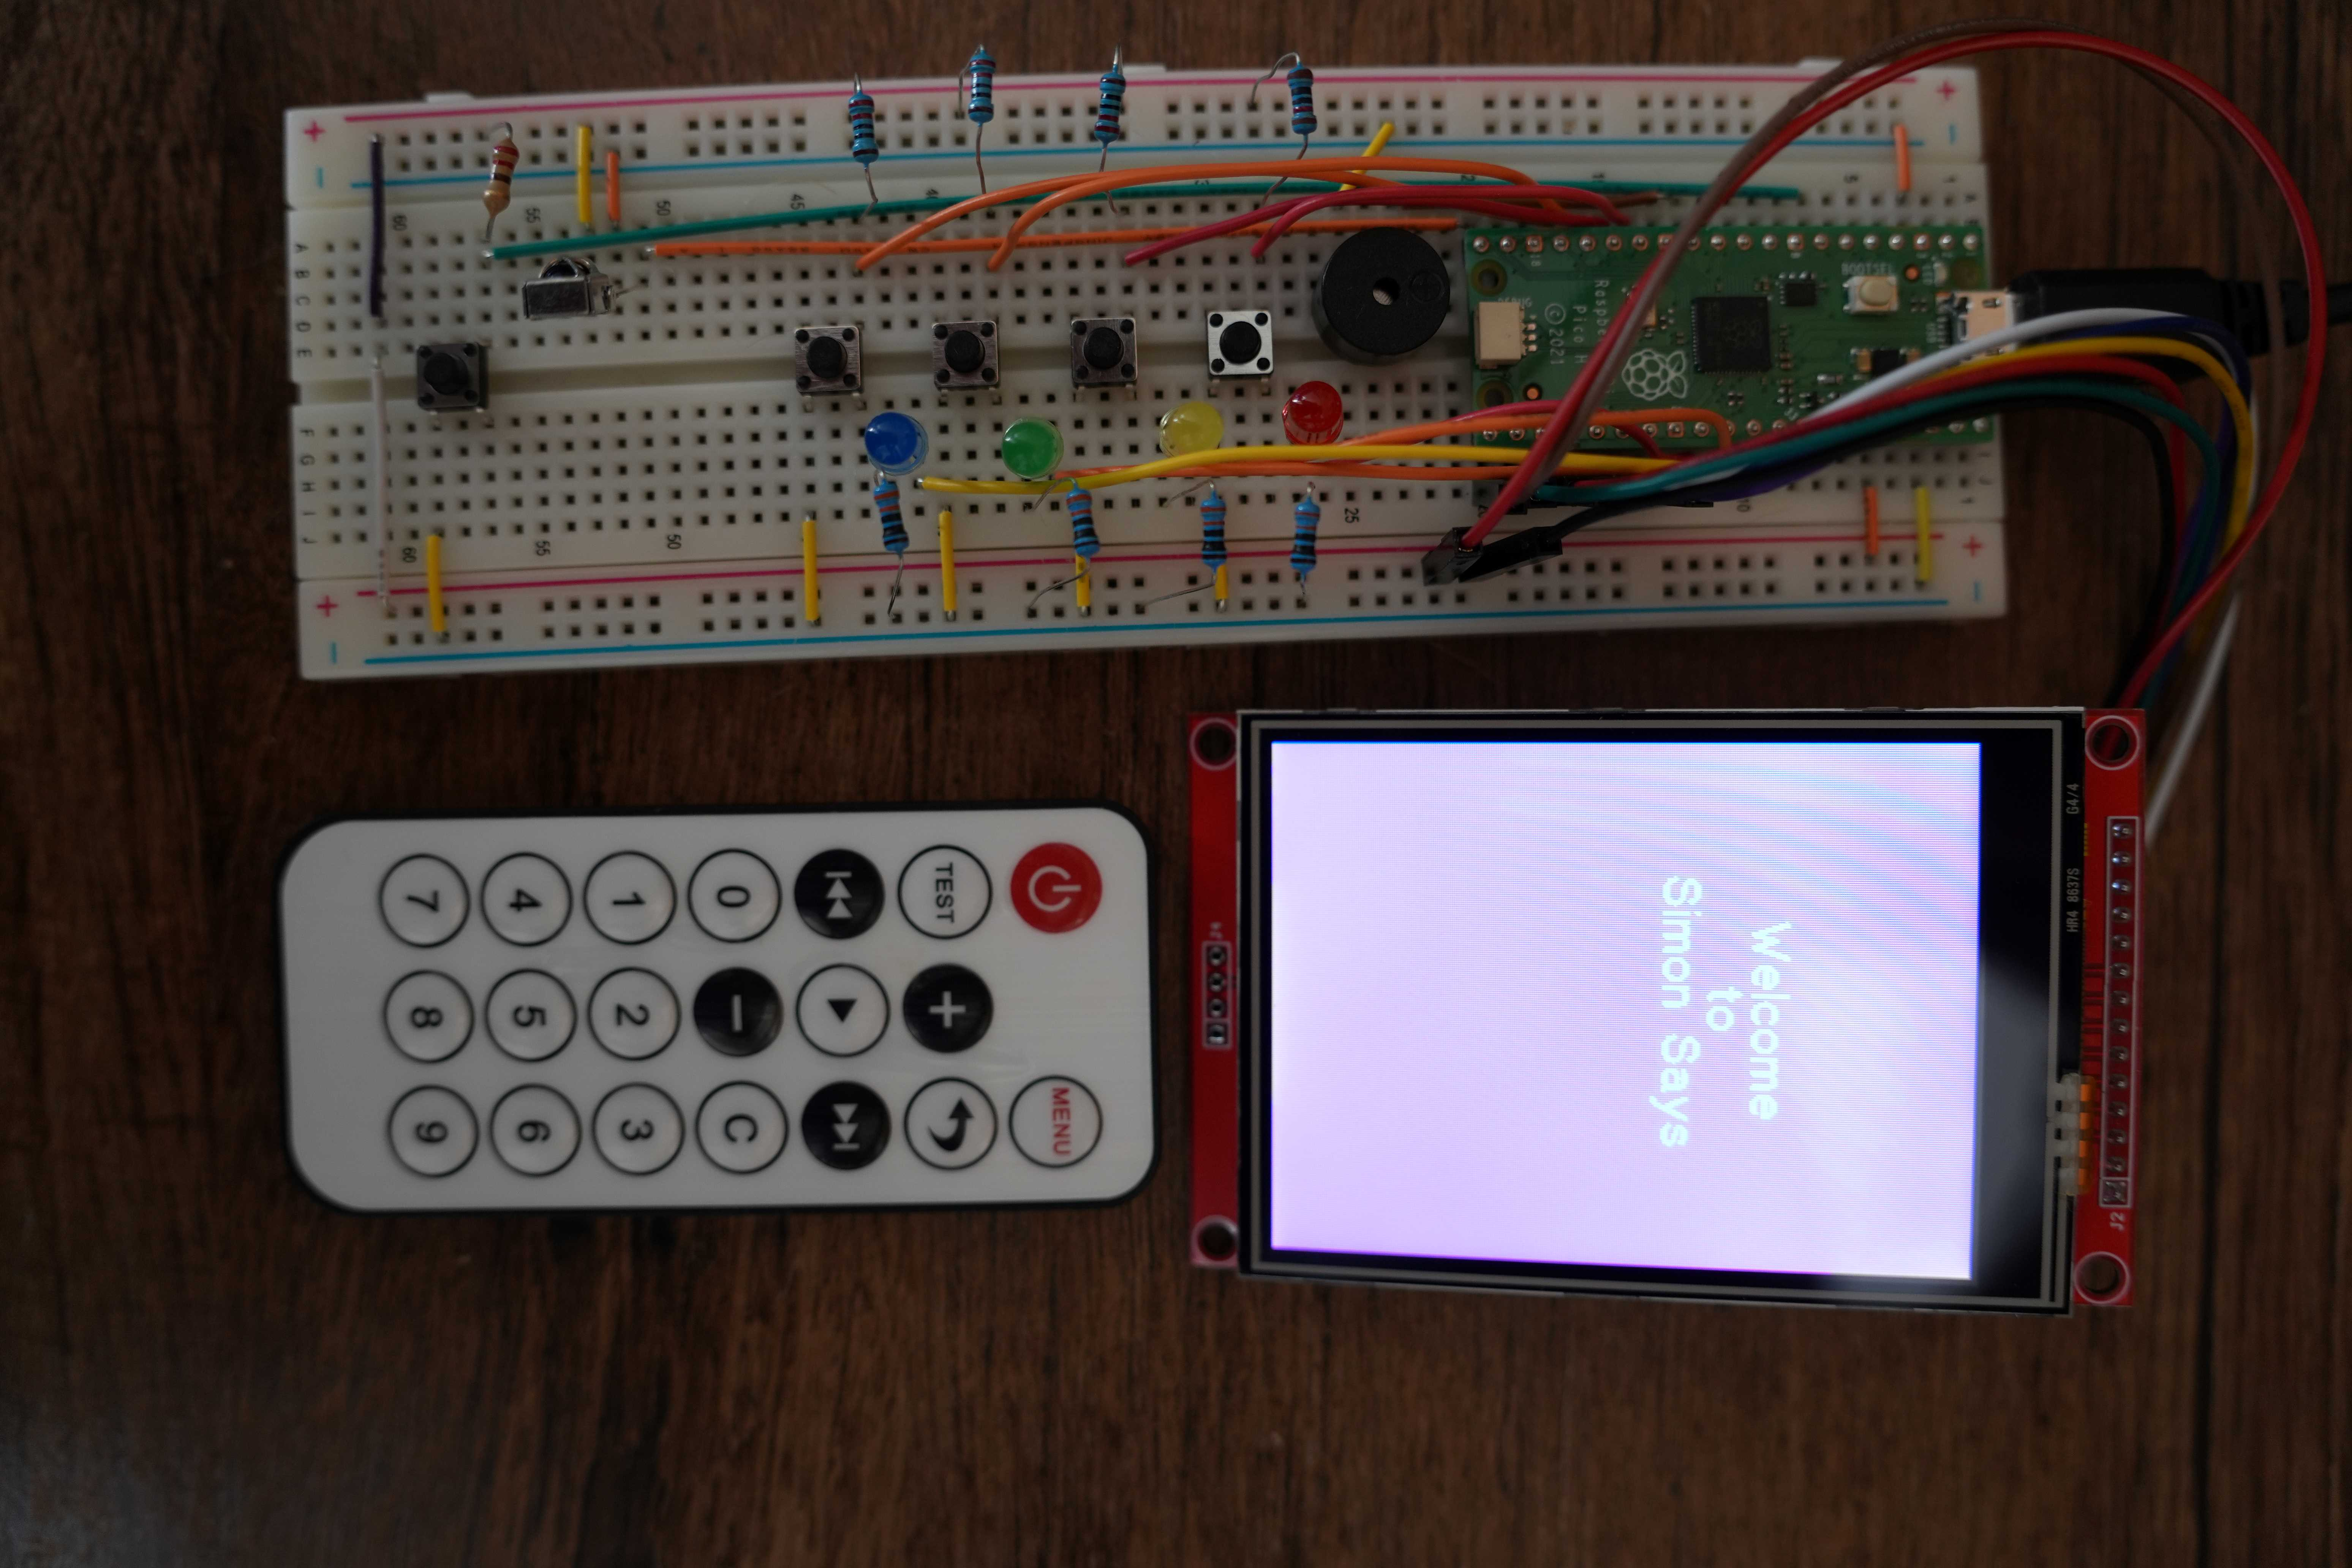
\includegraphics[width=\textwidth]{simon_says_compressed.jpg}
    \centering
    \caption{Hardware for Simon Says Game}
    \centering
    \label{fig:simon_says}
\end{figure}

Since no new assignments are being added to the class, the learning objectives for the 
class do not change.

\section{Project Deliverables}

In the GitHub repository associated with this paper, which can be found in Appendix
\ref{appendix:appendix_github}, the folder titled ``6-computer-applications-in-me'' 
contains the rewritten lab assignment, code skeleton, and solution for the exercise
mentioned above. The folder also contains a README that details what is in each file
and what software is needed to complete the assignments. Installation instructions can
be found in the ``usage-and-installation'' folder in the GitHub repository.

The integration of these curriculum changes would not be a simple task. Since the 
entire class is structured around C++ and the ESP32, every lecture, assignment, quiz,
and test would have to be translated. In addition to this, new PCBs would need to be 
designed for use with the Pico. 
